\documentclass[a4paper]{article}
\usepackage{tikz}
\usepackage{geometry}
\usepackage{graphicx}
\usepackage{natbib}
\usepackage{amsmath}
\usepackage{amssymb}
\usepackage{amsthm}
\usepackage{paralist}
\usepackage{epstopdf}
\usepackage{tabularx}
\usepackage{longtable}
\usepackage{multirow}
\usepackage{multicol}
\usepackage[hidelinks]{hyperref}
\usepackage{fancyvrb}
\usepackage{algorithm}
\usepackage{algorithmic}
\usepackage{float}
\usepackage{paralist}
%\usepackage[svgname]{xcolor}
\usepackage{enumerate}
\usepackage{array}
\usepackage{times}
\usepackage{url}
\usepackage{fancyhdr}
\usepackage{comment}
\usepackage{environ}
\usepackage{times}
\usepackage{textcomp}
\usepackage{caption}
\usepackage{bbm}
\usepackage{subcaption}


\urlstyle{rm}

\setlength\parindent{0pt} % Removes all indentation from paragraphs
\theoremstyle{definition}
\newtheorem{definition}{Definition}[]
\newtheorem{conjecture}{Conjecture}[]
\newtheorem{example}{Example}[]
\newtheorem{theorem}{Theorem}[]
\newtheorem{lemma}{Lemma}
\newtheorem{proposition}{Proposition}
\newtheorem{corollary}{Corollary}

\floatname{algorithm}{Procedure}
\renewcommand{\algorithmicrequire}{\textbf{Input:}}
\renewcommand{\algorithmicensure}{\textbf{Output:}}
\newcommand{\abs}[1]{\lvert#1\rvert}
\newcommand{\norm}[1]{\lVert#1\rVert}
\newcommand{\RR}{\mathbb{R}}
\newcommand{\CC}{\mathbb{C}}
\newcommand{\Nat}{\mathbb{N}}
\newcommand{\br}[1]{\{#1\}}
\DeclareMathOperator*{\argmin}{arg\,min}
\DeclareMathOperator*{\argmax}{arg\,max}
\renewcommand{\qedsymbol}{$\blacksquare$}

\definecolor{dkgreen}{rgb}{0,0.6,0}
\definecolor{gray}{rgb}{0.5,0.5,0.5}
\definecolor{mauve}{rgb}{0.58,0,0.82}

\definecolor{C0}{HTML}{1F77B4}
\definecolor{C1}{HTML}{FF7F0E}
\definecolor{C2}{HTML}{2ca02c}
\definecolor{C3}{HTML}{d62728}
\definecolor{C4}{HTML}{9467bd}
\definecolor{C5}{HTML}{8c564b}
\definecolor{C6}{HTML}{e377c2}
\definecolor{C7}{HTML}{7F7F7F}
\definecolor{C8}{HTML}{bcbd22}
\definecolor{C9}{HTML}{17BECF}

\newcommand{\Var}{\mathrm{Var}}
\newcommand{\Cov}{\mathrm{Cov}}
\newcommand{\sgn}{\mathrm{sgn}}

\newcommand{\vc}[1]{\boldsymbol{#1}}
\newcommand{\xv}{\vc{x}}
\newcommand{\Sigmav}{\vc{\Sigma}}
\newcommand{\alphav}{\vc{\alpha}}
\newcommand{\muv}{\vc{\mu}}

\newcommand{\red}[1]{\textcolor{red}{#1}}

\def\x{\mathbf x}
\def\y{\mathbf y}
\def\w{\mathbf w}
\def\v{\mathbf v}
\def\E{\mathbb E}
\def\R{\mathbb R}
\def\V{\mathbb V}
\def\ind{\mathbbm 1}

% TO SHOW SOLUTIONS, include following (else comment out):
\newenvironment{soln}{
    \leavevmode\color{blue}\ignorespaces
}{}


\hypersetup{
%    colorlinks,
    linkcolor={red!50!black},
    citecolor={blue!50!black},
    urlcolor={blue!80!black}
}

\geometry{
  top=1in,            % <-- you want to adjust this
  inner=1in,
  outer=1in,
  bottom=1in,
  headheight=3em,       % <-- and this
  headsep=2em,          % <-- and this
  footskip=3em,
}


\pagestyle{fancyplain}
\lhead{\fancyplain{}{Homework 7}}
\rhead{\fancyplain{}{CS 760 Machine Learning}}
\cfoot{\thepage}

\title{\textsc{Homework 7}} % Title

%%% NOTE:  Replace 'NAME HERE' etc., and delete any "\red{}" wrappers (so it won't show up as red)

\author{
\red{APOORVA KUMAR} \\
\red{908 461 5997}\\
} 

\date{}

\begin{document}

\maketitle 

\textbf{Instructions:}
Use this latex file as a template to develop your homework. Please submit a single pdf to Canvas. Late submissions may not be accepted. You can choose any programming language (i.e. python, R, or MATLAB). Please check Piazza for updates about the homework.
\vspace{0.1in}

\section{Kernel SVM [15 pts]}
Consider the following kernel function defined over $z,z'\in Z$:
\begin{align*}
k(z,z') =
\begin{cases}
1 & \text{~if~} z=z', \\
0 & \text{~otherwise.}
\end{cases}
\end{align*}
\begin{enumerate}
\item (5 pts) Prove that for any integer $m>0$, any $z_1, \ldots, z_m \in Z$, the $m \times m$ kernel matrix $K=[K_{ij}]$ is positive semi-definite, where $K_{ij}=k(z_i, z_j)$ for $i,j=\{1\ldots m\}$. (Let us assume that for $i \neq j$, we have $z_i \neq z_j$.)

\begin{soln}
    The Kernal Gram Matrix with the condition $z_i\neq z_j$ for $i\neq j$ is an $m\times m$ Indentity Matrix:
    $$
        \begin{bmatrix}
            1 & 0 & 0 & 0 & \hdots & 0 \\
            0 & 1 & 0 & 0 & \hdots & 0 \\
            0 & 0 & 1 & 0 & \hdots & 0 \\
            \vdots & \vdots & \vdots & \vdots & \ddots & \vdots \\
            0 & 0 & 0 & 0 & \hdots & 1 \\
        \end{bmatrix}
    $$
    To show that our Kernel matrix is positive semidefinte if $\forall v \in \mathbb R^{m}$ we have $ v^TKv \geq 0$ \\
    Now for $K=I_{m \times m}$ we get
    $$
        v^TIv=\sum^m_{i=1}v_i^2 \geq 0
    $$
    Hence we can conclude our Kernel is positive semidefinite.
\end{soln}

\item (5 pts) Given a training set $(z_1, y_1), \ldots, (z_n, y_n)$ with binary labels, the dual SVM problem with the above kernel $k$ will have parameters $\alpha_1, \ldots, \alpha_n, b \in \R$.  (Assume that for $i \neq j$, we have $z_i \neq z_j$.) The predictor for input $z$ takes the form
$$f(z) = \sum_{i=1}^n \alpha_i y_i k(z_i, z) + b.$$
Recall the label prediction is $\sgn(f(z))$.
Prove that there exists $\alpha_1, \ldots, \alpha_n, b$ such that $f$ correctly separates the training set.
In other words, $k$ induces a feature space rich enough such that in it any training set can be linearly separated.

\begin{soln}
    For any element $(z_i,y_i)$ in the training data where $y_i \in \{1,-1\}$:
    \begin{align*}
        f(z) & = \sum_{i=1}^n \alpha_i y_i k(z_i, z) + b \\
        & = \alpha_i y_i +b \\
        \sgn(f(z)) & = \sgn(\alpha_i y_i +b) \\
        \hat{y_i} &= \left\{
                        \begin{array}{ll}
                            \alpha_i + b  & y_i = 1 \\
                            -\alpha_i + b & y_i = -1
                        \end{array}
                    \right.
    \end{align*}
    Thus setting $\alpha_i > b$ for $y_i=1$ and $\alpha_i < b$ for $y_i=-1$ we can perfectly separate the data because $\alpha_i$ doesn't affect any other data point for $i\neq j$.
\end{soln}

\item (5 pts) How does that $f$ predict input $z$ that is not in the training set?

\begin{soln}
    For any $z \notin {(z_i)}_{i=1}^n$
    $$
        k(z,z_i)=0\;\forall\,i=\{1,2,...,n\}
    $$
    Thus,
    $$
        \sgn(f(z)) = \sgn(b)
    $$
    So, we can see that for any $z$ not in training set have $\hat{y}=\sgn(b)$.
\end{soln}

\end{enumerate}

Comment: One useful property of kernel functions is that the input space $Z$ does not need to be a vector space; in other words, $z$ does not need to be a feature vector.  For all we know, $Z$ can be turkeys in the world.  As long as we can compute $k(z,z')$, kernel SVM works on turkeys.

\section{Game of Classifiers [50 pts]}
 \subsection{Implementation}
  Implement the following models in choice of your programming language. Include slack variables in SVM implementation if needed. You can use autograd features of pytorch, tensorflow etc. or derive gradients on your own. (But don't use inbuilt models for SVM, Kernel SVM and Logistic Regression from libraries)
  
  \begin{itemize}
      \item Implement Linear SVM (without kernels). 
      \item Implement Kernel SVM, with options for linear, rbf and polynomial kernels. You should keep the kernel parameters tunable (e.g. don't fix the degree of polynomial kernels but keep it as a variable and play with different values of it. Is Linear SVM a special case of Kernel SVMs?
      
      \begin{soln}
          Yes, Linear SVM is a special case of Kernel SVM.
      \end{soln}
      \item Implement Logistic Regression with and without kernels (use same kernel as Question 1).
      
  \end{itemize}
 \subsection{Evaluation on Synthetic Dataset}
 \subsubsection{Synthetic Dataset-1 (20 pts)}
 Generate 2-D dataset as following, \\
 Let $\mu=2.5$ and $I_2$ be the $2\times2$ identity matrix. Generate points for the positive and negative classes respectively from $\mathcal{N}([\mu,0],I_2)$, and $\mathcal{N}([-\mu,0],I_2)$. For each class generate 750 points, (1500 in total). Randomly create train, validation and test splits of size 1000, 250, 250 points respectively. Do the following with this dataset:
 \begin{itemize}
     \item (5 pts) Train your Linear SVM, Logistic Regression models and report decision boundaries, test accuracies. 
     \begin{soln}
         SVM Test Accuracy: 99.6\% \\
         Logistic Regression Test Accuracy: 99.6\%
         \begin{figure}[H]
            \centering
            \begin{subfigure}[b]{0.5\textwidth}
                \centering
                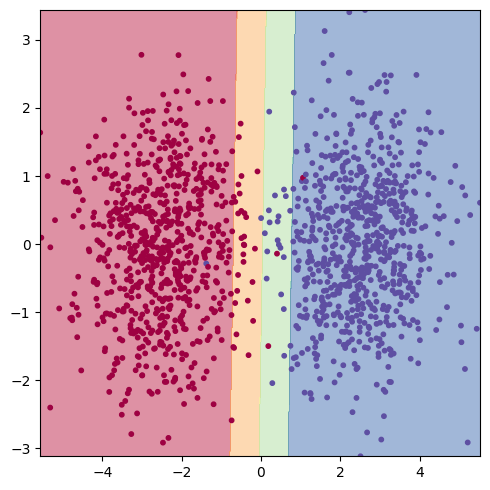
\includegraphics[scale=0.3]{Images/q2_2_1/SVM.png}
                \caption{SVM}
            \end{subfigure}%
            \begin{subfigure}[b]{0.5\textwidth}
                \centering
                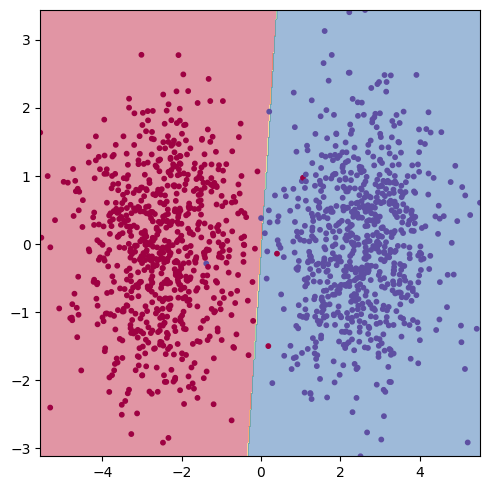
\includegraphics[scale=0.3]{Images/q2_2_1/Logistic.png}
                \caption{Logistic Regression}
            \end{subfigure}
            \caption{Decision Boundaries}
        \end{figure}
     \end{soln}
     \item (5 pts) Show decision boundaries with K-NN and Naive Bayes Classifiers. ( You can use library implementations or implement from scratch. Figure out the hyper-parameters using the validation set.) 
     
     \begin{soln}
         KNN Test Accuracy for \textbf{K=3} = 100\% \\
         Naive Bayes Test Accuracy for smoothing parameter as 1 = 99.2\%
         \begin{figure}[H]
            \centering
            \begin{subfigure}[b]{0.5\textwidth}
                \centering
                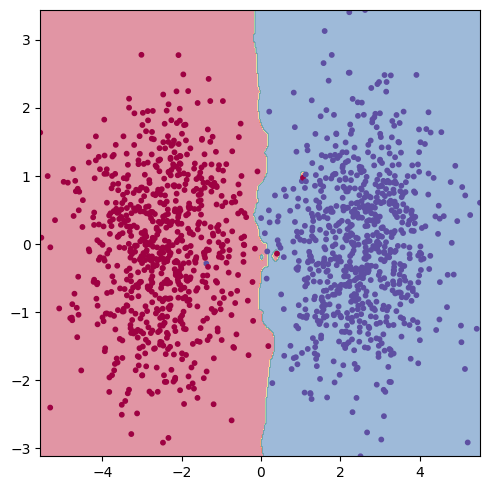
\includegraphics[scale=0.3]{Images/q2_2_1/KNN.png}
                \caption{KNN}
            \end{subfigure}%
            \begin{subfigure}[b]{0.5\textwidth}
                \centering
                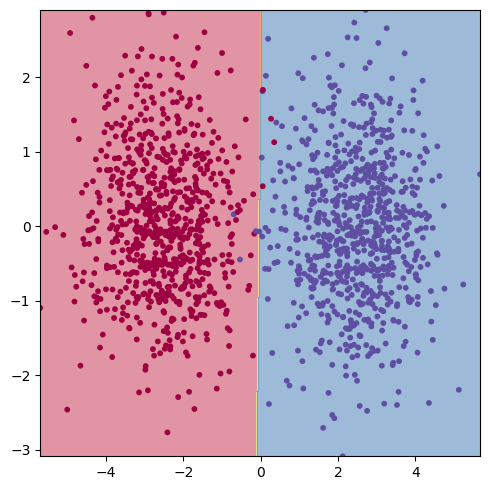
\includegraphics[scale=0.3]{Images/q2_2_1/Niave.png}
                \caption{Naive Bayes}
            \end{subfigure}
            \caption{Decision Boundaries}
        \end{figure}
     \end{soln}
     \item (5 pts) Repeat the process by varying $\mu$ from 1.0 to 2.4 with step size of 0.2, for each value of $\mu$ obtain test accuracies of the models and plot ( $\mu$ on x-axis and test accuracy on y-axis). ( You will have a curve for each of the 4-classifiers mentioned above)
     \begin{figure}[H]
         \centering
         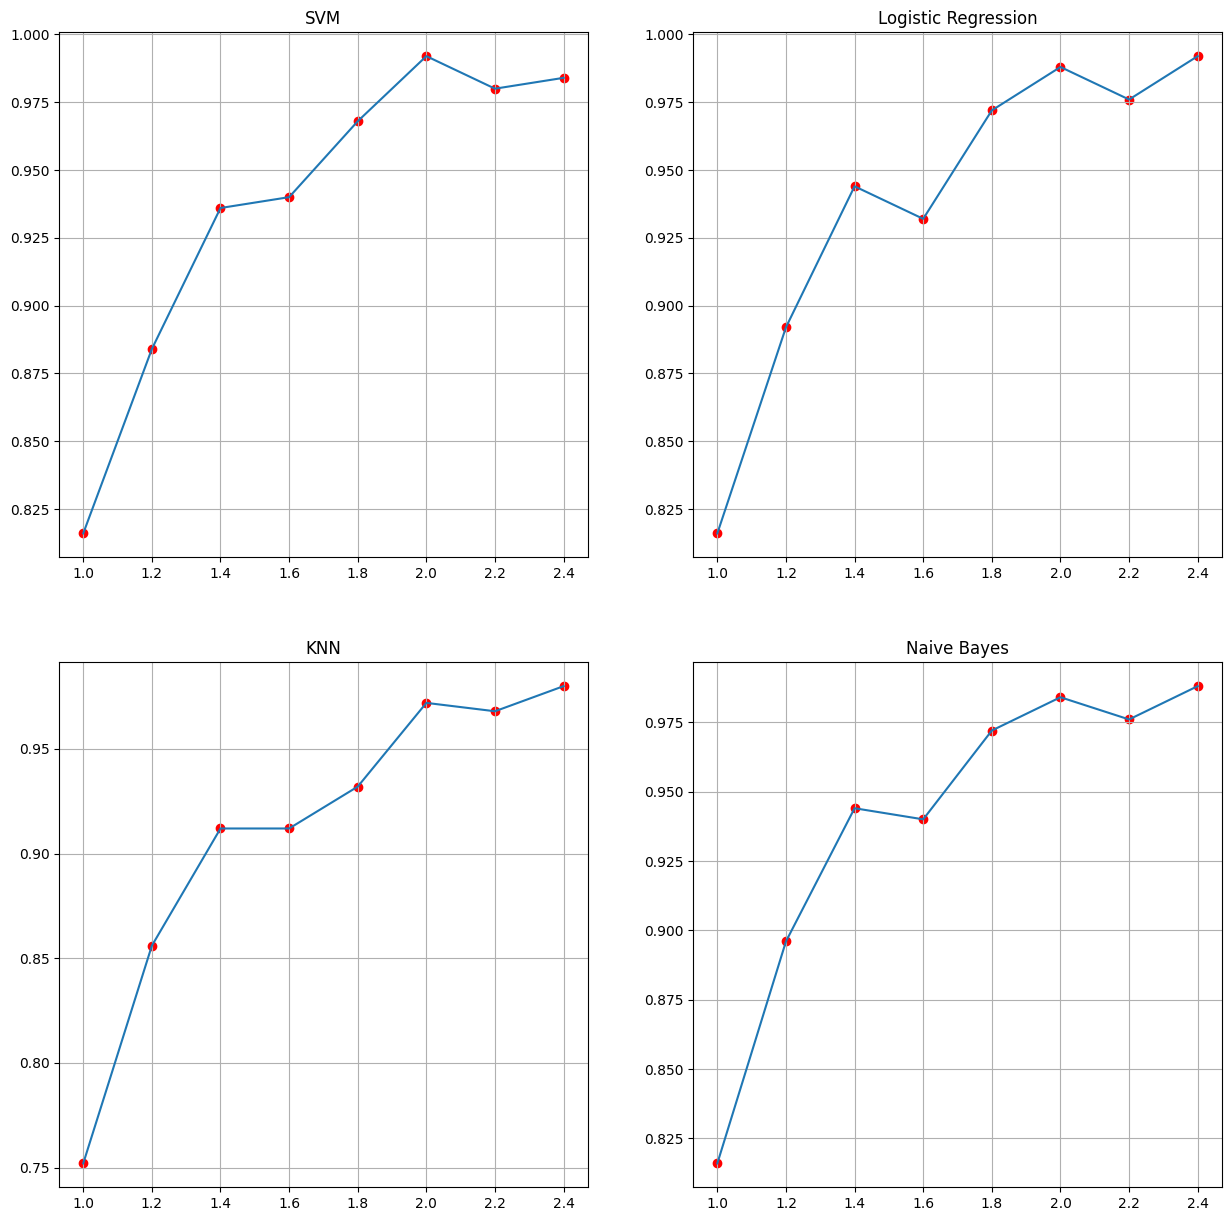
\includegraphics[scale=0.3]{Images/q2_2_1/all.png}
     \end{figure}
     \item (5 pts) What are your conclusions from this exercise?
     
     \begin{soln}
         As $\mu$ increase the data becomes more seperable and it becomes much easier to classifier the data. We also see that all of them form almost a linear decision boundary even including the KNN classifier.
     \end{soln}
 \end{itemize}
 
 \subsubsection{Synthetic Dataset-2  (20 pts) }
 Generate 1500 data points from the 2-D circles dataset of sklearn (\texttt{sklearn.datasets.make\_circles}). Randomly create train, validation and test splits of size 1000, 250, 250 points respectively. Evaluate the above classifiers on this setting.
 \begin{itemize}
     \item (5 pts) Show decision boundaries for Linear SVM and Logistic Regression classifiers. 

     \begin{soln}
        Linear SVM has 60.33 \% and Logistic has 32.33 \% test accuracy.
         \begin{figure}[H]
                \centering
                \begin{subfigure}[b]{0.5\textwidth}
                    \centering
                    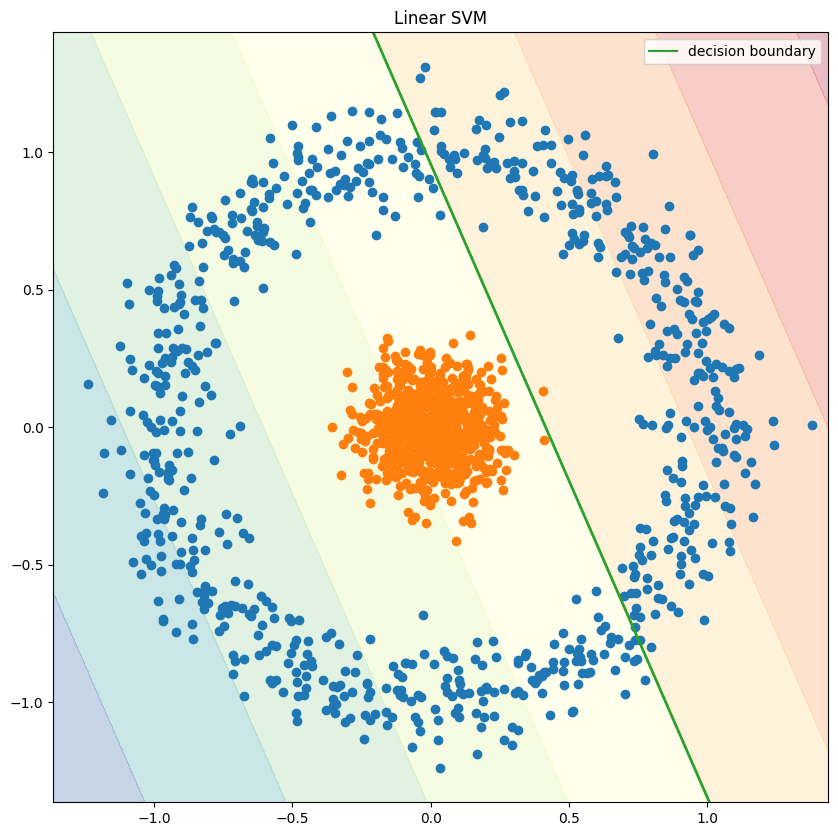
\includegraphics[scale=0.2]{Images/q2_2_2/SVM_Linear.png}
                    \caption{Linear SVM}
                \end{subfigure}%
                \begin{subfigure}[b]{0.5\textwidth}
                    \centering
                    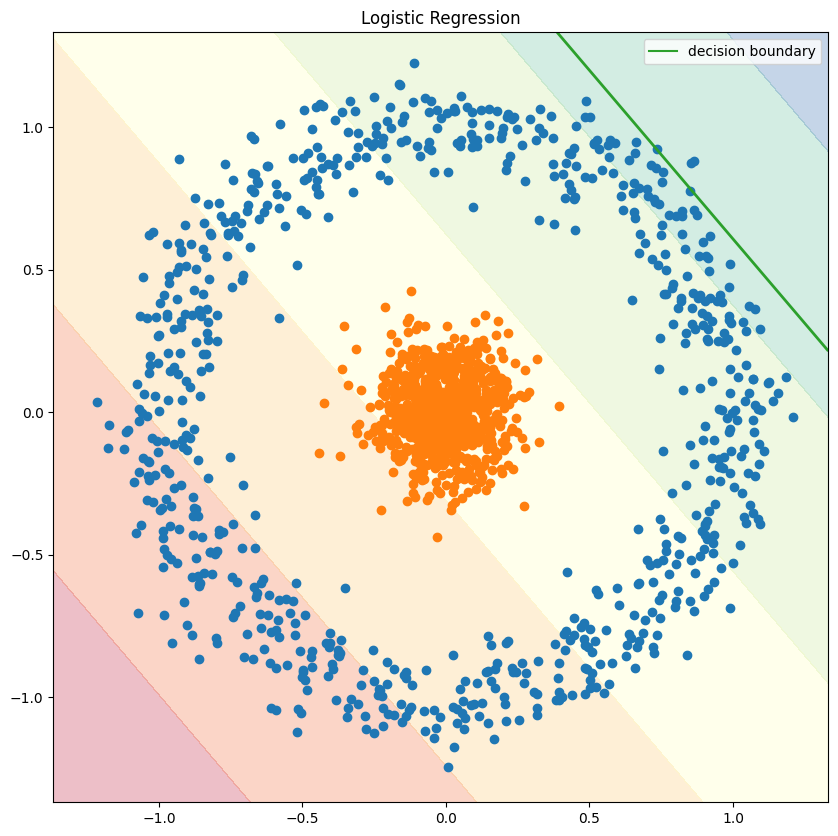
\includegraphics[scale=0.2]{Images/q2_2_2/Log_Lin.png}
                    \caption{Logistic Regression}
                \end{subfigure}
                \caption{Decision Boundaries}
            \end{figure}
     \end{soln}
        
     \item (5 pts) Show decision boundaries for Kernel SVM and Kernel Logistic Regression (use rbf, polynomial kernels). Try different values of hyperparameters, report results with whichever works the best.
     
     \begin{soln}
        All of these have 100\% test accuracy.
         \begin{figure}[H]
            \centering
            \begin{subfigure}[b]{0.5\textwidth}
                \centering
                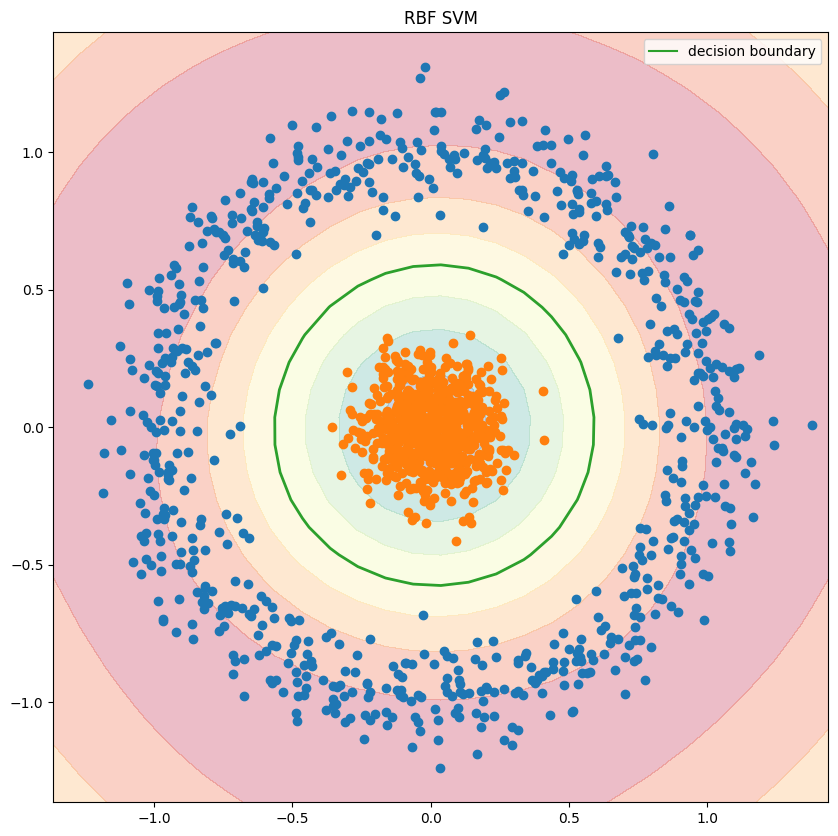
\includegraphics[scale=0.2]{Images/q2_2_2/SVM_RBF.png}
                \caption{SVM}
            \end{subfigure}%
            \begin{subfigure}[b]{0.5\textwidth}
                \centering
                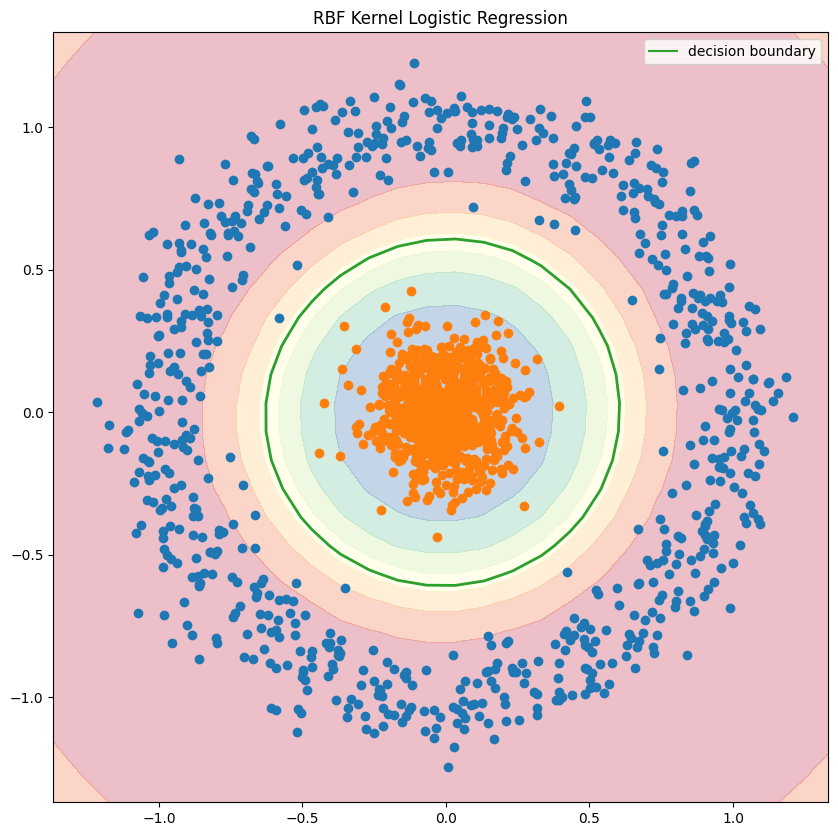
\includegraphics[scale=0.2]{Images/q2_2_2/Log_RBF.png}
                \caption{Logistic Regression}
            \end{subfigure}
            \caption{Decision Boundaries for RBF Kernel}
        \end{figure}
        \begin{figure}[H]
            \centering
            \begin{subfigure}[b]{0.5\textwidth}
                \centering
                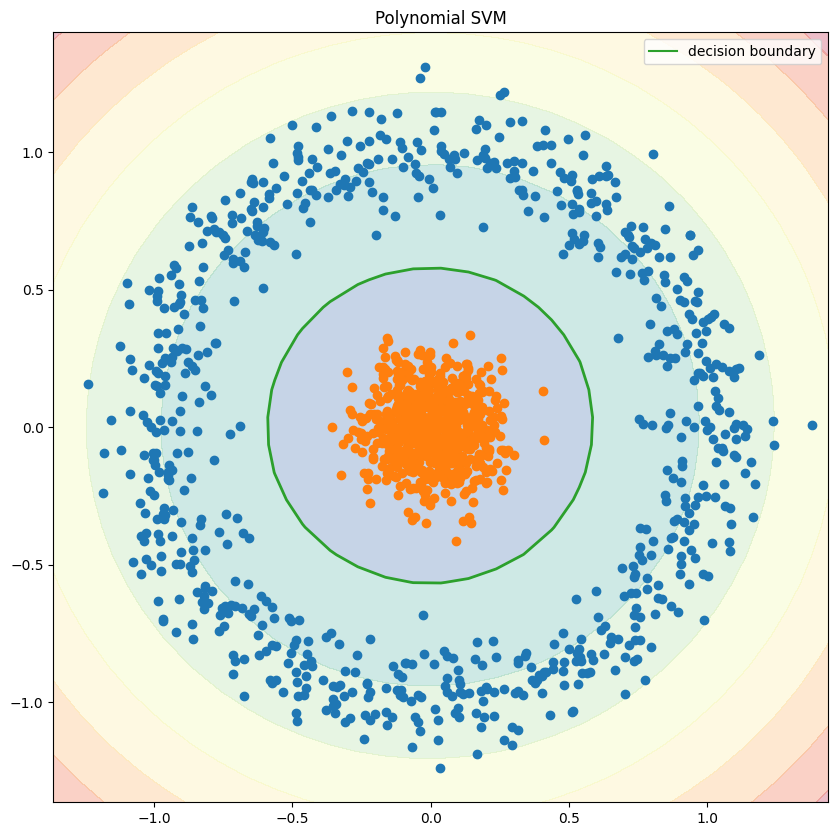
\includegraphics[scale=0.2]{Images/q2_2_2/SVM_Poly.png}
                \caption{SVM}
            \end{subfigure}%
            \begin{subfigure}[b]{0.5\textwidth}
                \centering
                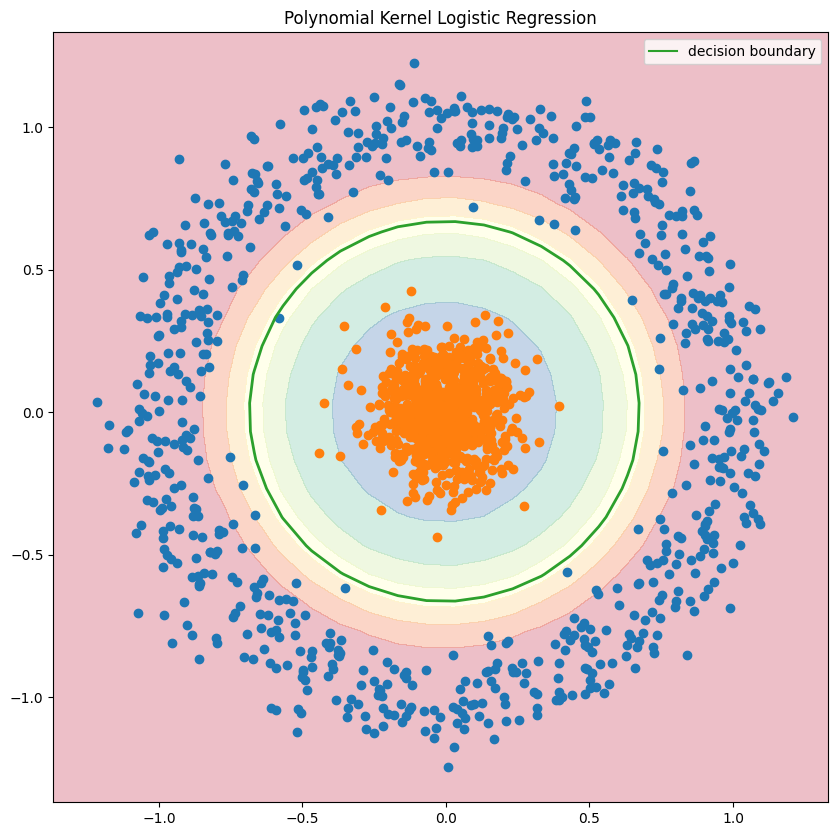
\includegraphics[scale=0.2]{Images/q2_2_2/Log_Poly.png}
                \caption{Logistic Regression}
            \end{subfigure}
            \caption{Decision Boundaries for Polynomial Kernel}
        \end{figure}
     \end{soln}
     
     \item (5 pts) Train Neural Network from HW4, and K-NN classifiers on this dataset and show decision boundaries. (You can use library implementation for these classifiers).
     
     \begin{soln}
        Both have 100\% test accuracy
         \begin{figure}[H]
            \centering
            \begin{subfigure}[b]{0.5\textwidth}
                \centering
                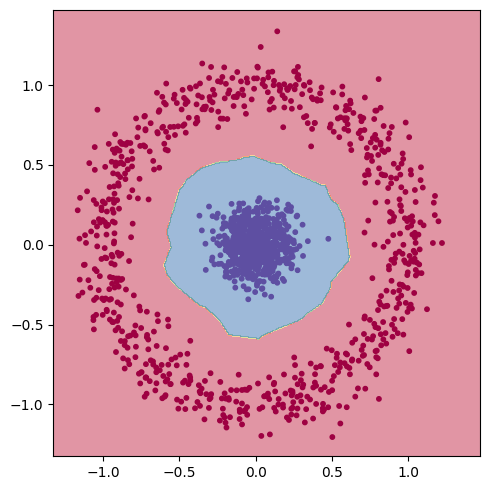
\includegraphics[scale=0.3]{Images/q2_2_3/KNN.png}
                \caption{KNN}
            \end{subfigure}%
            \begin{subfigure}[b]{0.5\textwidth}
                \centering
                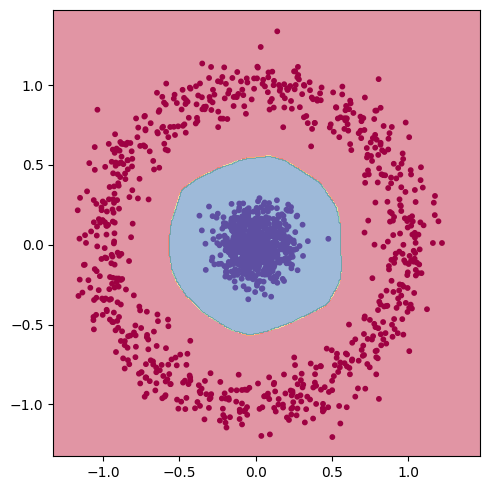
\includegraphics[scale=0.3]{Images/q2_2_3/NeuralNet.png}
                \caption{Neural Network}
            \end{subfigure}
            \caption{Decision Boundaries}
        \end{figure}
        
     \end{soln}
     
     \item (5 pts) What are your conclusions from this exercise?
     
     \begin{soln}
         We see that for a dataset which is not linearly separable, kernels help a lot to ease the process by projecting the dataset in a space where it can be easily classified. This eases our process a lot wherein we can just plug and play a kernel into the process.
     \end{soln}
 \end{itemize}
 
 \subsection{Evaluation on Real Dataset (10 pts)}
 Lets put all this to some real use. For this problem use the the Wisconsin Breast Cancer dataset. You can download it from sklearn library(\texttt{sklearn.datasets.load\_breast\_cancer)
}
\begin{itemize}
    \item (5 pts) Do all the points of section 2.2.2 on this dataset. Since this is high-dimensional data, so you don't have to show the decision boundaries. Just report test accuracies for these classifiers and discuss your findings.
    
    \begin{soln}
        Data was split into 369 samples for training, 100 for validation and 100 for testing.
        \begin{center}
            \begin{tabular}{|c|c|}
                \hline
                Model Name & Test Accuracy \\
                \hline
                Linear SVM & 62\% \\
                RBF SVM & 89\% \\
                Polynomial SVM (p=5) & 76\% \\
                Logistic Regression & 62\% \\
                RBF Logistic Regression & 62\% \\
                Polynomial Logistic Regression (p=10) & 62\% \\
                KNN(k=6) & 90\% \\
                Neural Network & 92\% \\
                \hline
            \end{tabular}
        \end{center}
    \end{soln}
    
    \item (5 pts) In addition, you also want to figure out the  important features which determine the class. Which regularization will you use for this? Upgrade your SVM, Kernel SVM implementation to include this regularization. Discuss what are the important features that you obtain by running your regularized SVM on this dataset. (You might have to normalize this dataset before training any classifier).
    
    \begin{soln}
        Test Losses for Regularized SVM:
        \begin{enumerate}
            \item Linear = 62 \%
            \item Polynomial = 78 \%
            \item RBF = 91 \%
        \end{enumerate}
        The important features chosen were: ['mean perimeter', 'mean area', 'mean smoothness', 'mean concavity', 'texture error', 'concavity error', 'concave points error', 'worst perimeter', 'worst area', 'worst concavity', 'worst fractal dimension']
    \end{soln}
\end{itemize}

\section{VC dimension [20 pts]}
\begin{enumerate}
    \item (7 pts) Let the input $x\in \mathcal{X}=\R$.
Consider $\mathcal{F}=\{f(x)=\sgn(ax^2+bx+c): a, b, c \in \R\}$, where $\sgn(z)=1$ if $z\ge0$, and 0 otherwise.
What is $VC(\mathcal{F})$?  Prove it.

\subsection*{Shatter Coefficient and VC dimension}
The main intuition behind VC theory is that, although a collection of classifiers may be infinite, using a finite set of training data to select a good rule effectively reduces the number of different classifiers we need to consider. We can measure the effective size of class $\mathcal{F}$ using \textit{shatter coefficient}. Suppose we have a training set $D_n = \{(x_i, y_i)\}_{i=1}^n$ for a binary classification problem with labels $y_i = \{-1, +1\}$. Each classifier in $\mathcal{F}$ produces a binary label sequence
$$\big(f(x_1), \cdots, f(x_n)\big) \in \{-1, +1\}^n$$
There are at most $2^n$ distinct sequences, but often no all sequences can be generated by functions in $\mathcal{F}$. Shatter coefficient $\mathcal{S}(\mathcal{F}, n)$ is defined as the maximum number of labeling sequences the class $\mathcal{F}$ induces over $n$ training points in the feature space $\mathcal{X}$. More formally, 
$$\mathcal{S}(\mathcal{F}, n) = \max_{x_1, \cdots, x_n \in \mathcal{X}}
\Bigg|\Big\{\big(f(x_1), \cdots, f(x_n)\big)\Big\} \in \{-1, +1\}^n, f \in \mathcal{F}\Bigg|$$
where $|\cdot|$ denotes the number of elements in the set.
The \textit{Vapnik-Chervonenkis (VC) dimension} $V(\mathcal{F})$ of a class $\mathcal{F}$  is defined as the largest integer $k$ such that $\mathcal{S}(\mathcal{F}, k) = 2^k$.

\begin{soln}
    We move down the values of $k$ until we find a $k$ where $\mathcal S(\mathcal F,k)\neq 2^k$.
    \begin{itemize}
        \item $\mathbf{k=1}, (x_1)$: Easily classifiable into $\{(+),(-)\}$, Thus $\mathcal S=2$
        \item $\mathbf{k=2}, (x_1\leq x_2)$: Easily classifiable into $\{(++),(--)\}$
            \begin{itemize}
                \item For $(+-)$ use $f(x)=\sgn((x-(x_2+1))(x-\frac{x_1+x_2}{2}))$
                \item For $(-+)$ use $f(x)=\sgn((x-(x_1-1))(x-\frac{x_1+x_2}{2}))$
            \end{itemize}
            Thus $\mathcal S=4$
        \item $\mathbf{k=3}, (x_1\leq x_2\leq x_3)$: Easily classifiable into $\{(+++),(---)\}$
            \begin{itemize}
                \item For $(++-)$ use $f(x)=\sgn((x-(x_3+1))(x-\frac{x_2+x_3}{2}))$
                \item For $(+-+)$ use $f(x)=\sgn((x-\frac{x_1+x_2}{2})(x-\frac{x_2+x_3}{2}))$
                \item For $(-++)$ use $f(x)=\sgn((x-(x_1-1))(x-\frac{x_1+x_2}{2}))$
                \item For $(+--)$ use $f(x)=\sgn((x-\frac{x_1+x_2}{2})(x-(x_3+1)))$
                \item For $(--+)$ use $f(x)=\sgn((x-(x_1-1))(x-\frac{x_2+x_3}{2}))$
                \item For $(-+-)$ use use $f(x)=\sgn((\frac{x_1+x_2}{2}-x)(x-\frac{x_2+x_3}{2}))$
            \end{itemize}
            Thus $\mathcal S=8$
        \item $\mathbf{k=4}, (x_1\leq x_2\leq x_3\leq x_4)$: Here we see that using the form $f(x)=\sgn(ax^2+bx+c)$ we can't classify $(+-+-)$ in any way possible.
    \end{itemize}
    Therefore, $VC(\mathcal F)=3$
\end{soln}

\item (7 pts) Suppose there are $n$ points $(x_1, \cdots, x_n)\in\R$. Let $\mathcal{F}$ be the collection of 1-d linear classifiers: for each $t\in [0, 1], f_t \in \mathcal{F}$ labels $x\leq t$ as $-1$ and $x > t$ as $+1$, or vice-versa. What is the shatter coefficient $S(\mathcal{F}, n)$? What is VC-dimension $V(\mathcal{F})$? How can you get it from shatter coefficient?

\begin{soln}
    The above mentioned $\mathcal F$ is a classifier, classifying all points to the left of it as $-1$ and all to right of it as $+1$.
    
    Lets arrange the points in a sequence $(x_{1'},x_{2'},...x_{n'})$ where $x_{i'}\leq x_{j'}\;\forall\;i'<j'$. Using this we can show that:
    $$\mathcal S(\mathcal F,n)=n+1$$
    This comes from the fact that the different ways to place a 1-d linear classifier is:
    \begin{itemize}
        \item $n-1$ regions between the n sequentially arranged points
        \item 2 classifier on the extreme ends of the data-points i.e. $t<x_{1'}$ and $t>x_{n'}$
    \end{itemize} 
    making a total $\mathbf{n+1}$ 1-d classifier's.

    The VC dimension: $$VC(\mathcal F)=1$$ for this definition of $\mathcal F$.
    
    This can be calculated by equating $\mathcal S(\mathcal F,n)=n+1=2^n$ and solving gives us $\mathbf{n=1}$
\end{soln}
\item (6 pts) Show the following monotonicity property of VC-dimension: if $\mathcal{F}$ and $\mathcal{F}'$ are hypothesis classes with $\mathcal{F} \subset \mathcal{F}'$, then the VC-dimension of $\mathcal{F}'$ is greater than or equal to that of $\mathcal{F}$.

\begin{soln}
    If $\mathcal F$ is a subset of $\mathcal F'$ then all the labelling sequences or shattering that are induced by class $\mathcal{F}$ are a part of $\mathcal{F'}$. Now considering $\mathcal F$ is a subset of $\mathcal F'$, $\mathcal F$ is some specific set of hypothesis class with tighter criteria to their form than $\mathcal F'$, hence $\mathcal F'$ with a looser form might be able to accommodate more labelling sequences or at-least have the same number of labelling sequences. Thus $\mathcal F'$ can have a higher VC-dimension or equivalent VC-dimension to $\mathcal F$ but never lower.

    If we assume $\mathcal F'$ has a lower VC-dimension than $\mathcal F$ then there is some shattering in $\mathcal F$ which $\mathcal F'$ can't produce for a given $n$. This directly contradicts the fact $\mathcal{F} \subset \mathcal{F}'$ because if $\mathcal F$ can shatter a sequence then $\mathcal F'$ should be able to do it too.
\end{soln}
\end{enumerate}

\section{Q-learning [15 pts]}
Consider the following Markov Decision Process.
It has two states $s$. It has two actions $a$: move and stay. The state transition is deterministic: ``move'' moves to the other state, while ``stay' stays at the current state. The reward $r$ is 0 for move,  1 for stay. There is a discounting factor $\gamma=0.8$.
\\

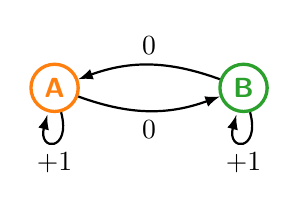
\begin{tikzpicture}
    \tikzstyle{n} = [very thick,circle,inner sep=0mm,minimum width=6mm]
    \tikzstyle{a} = [thick,>=latex,->]
    \def\dx{1.2}
    \def\dy{-1.2}
    \node[n,C1,draw=C1] (2) at (\dy,0) {\textbf{\textsf{A}}};
    \node[n,C2,draw=C2] (1) at (\dx,0) {\textbf{\textsf{B}}};
    \path[a]
    (2) edge [loop below] node {+1}(2)
    (1) edge [loop below] node {+1}(1)
    (2) edge [bend right=20] node[below] {0}(1)
    (1) edge [bend right=20] node[above] {0}(2);
\end{tikzpicture}

The reinforcement learning agent performs Q-learning.  Recall the $Q$ table has entries $Q(s,a)$. The $Q$ table is initialized with all zeros. The agent starts in state $s_1=A$. In any state $s_t$, the agent chooses the action $a_t$ according to a behavior policy $a_t = \pi_B(s_t)$. Upon experiencing the next state and reward $s_{t+1}, r_t$ the update is:
$$Q(s_t, a_t) \Leftarrow (1-\alpha) Q(s_t, a_t) + \alpha \left( r_t + \gamma \max_{a'} Q(s_{t+1}, a') \right).$$
Let the step size parameter $\alpha=0.5$.

\begin{enumerate}
\item (5 pts) Run Q-learning for 200 steps with a deterministic greedy behavior policy: at each state $s_t$ use the best action $a_t \in \argmax_a Q(s_t,a)$ indicated by the current Q table. If there is a tie, prefer move. Show the Q table at the end.

\begin{soln}
    \begin{center}
        \begin{tabular}{ | m{5em} | m{5em}| m{5em} |} 
          \hline
          Q Value & Move & Stay \\ 
          \hline
          A & 0 & 0  \\ 
          \hline
          B & 0 & 0\\ 
          \hline
        \end{tabular}
    \end{center}
\end{soln}

\item (5 pts) Reset and repeat the above, but with an $\epsilon$-greedy behavior policy: at each state $s_t$, with probability $1-\epsilon$ choose what the current Q table says is the best action: $\argmax_a Q(s_t,a)$; Break ties arbitrarily. Otherwise, (with probability $\epsilon$) uniformly chooses between move and stay (move or stay both with 1/2 probability). Use $\epsilon=0.5$.

\begin{soln}
    \begin{center}
            \begin{tabular}{ | m{5em} | m{5em}| m{5em} |} 
              \hline
              Q Value & Move & Stay \\ 
              \hline
              A & 3.972 & 4.999 \\ 
              \hline
              B & 3.998 & 4.977\\ 
              \hline
            \end{tabular}
        \end{center}
\end{soln}

\item (5 pts) Without doing simulation, use Bellman equation to derive the true Q table induced by the MDP.
\begin{soln}
    $$Q(s_t, a_t) \Leftarrow (1-\alpha) Q(s_t, a_t) + \alpha \left( r_t + \gamma \max_{a'} Q(s_{t+1}, a') \right).$$
    \begin{gather*}
        s_t=\{A,B\} \\
        a_t=\{\text{Stay},\text{Move}\}
    \end{gather*}
    $s_1=A$
    \begin{center}
        \begin{tabular}{ | m{5em} | m{5em}| m{5em} |} 
          \hline
          $Q_0$ & Move & Stay \\ 
          \hline
          A & 0 & 0  \\ 
          \hline
          B & 0 & 0\\ 
          \hline
        \end{tabular}
    \end{center}
    Choosing $1^{th}$ Action $a_{1} = \text{Move}$: $s_{2}=B\;,\;r_{1}=1\;,\;Q(A,\text{Move}) = 0.5$
        \begin{center}
            \begin{tabular}{ | m{5em} | m{5em}| m{5em} |} 
            \hline
            $Q_{1}$ & Move & Stay \\ 
            \hline
            A & 0.5 & 0  \\
            \hline
            B & 0 & 0 \\ 
            \hline
            \end{tabular}
        \end{center}
Choosing $2^{th}$ Action $a_{2} = \text{Stay}$: $s_{3}=B\;,\;r_{2}=0\;,\;Q(B,\text{Stay}) = 0.0$
        \begin{center}
            \begin{tabular}{ | m{5em} | m{5em}| m{5em} |} 
            \hline
            $Q_{2}$ & Move & Stay \\ 
            \hline
            A & 0.5 & 0  \\
            \hline
            B & 0 & 0.0 \\ 
            \hline
            \end{tabular}
        \end{center}
Choosing $3^{th}$ Action $a_{3} = \text{Move}$: $s_{4}=A\;,\;r_{3}=1\;,\;Q(B,\text{Move}) = 0.7$
        \begin{center}
            \begin{tabular}{ | m{5em} | m{5em}| m{5em} |} 
            \hline
            $Q_{3}$ & Move & Stay \\ 
            \hline
            A & 0.5 & 0  \\
            \hline
            B & 0.7 & 0.0 \\ 
            \hline
            \end{tabular}
        \end{center}
Choosing $4^{th}$ Action $a_{4} = \text{Stay}$: $s_{5}=A\;,\;r_{4}=0\;,\;Q(A,\text{Stay}) = 0.2$
        \begin{center}
            \begin{tabular}{ | m{5em} | m{5em}| m{5em} |} 
            \hline
            $Q_{4}$ & Move & Stay \\ 
            \hline
            A & 0.5 & 0.2  \\
            \hline
            B & 0.7 & 0.0 \\ 
            \hline
            \end{tabular}
        \end{center}
Choosing $5^{th}$ Action $a_{5} = \text{Move}$: $s_{6}=B\;,\;r_{5}=1\;,\;Q(A,\text{Move}) = 1.03$
        \begin{center}
            \begin{tabular}{ | m{5em} | m{5em}| m{5em} |} 
            \hline
            $Q_{5}$ & Move & Stay \\ 
            \hline
            A & 1.03 & 0.2  \\
            \hline
            B & 0.7 & 0.0 \\ 
            \hline
            \end{tabular}
        \end{center}
Choosing $6^{th}$ Action $a_{6} = \text{Stay}$: $s_{7}=B\;,\;r_{6}=0\;,\;Q(B,\text{Stay}) = 0.28$
        \begin{center}
            \begin{tabular}{ | m{5em} | m{5em}| m{5em} |} 
            \hline
            $Q_{6}$ & Move & Stay \\ 
            \hline
            A & 1.03 & 0.2  \\
            \hline
            B & 0.7 & 0.28 \\ 
            \hline
            \end{tabular}
        \end{center}
Choosing $7^{th}$ Action $a_{7} = \text{Stay}$: $s_{8}=B\;,\;r_{7}=0\;,\;Q(B,\text{Stay}) = 0.42$
        \begin{center}
            \begin{tabular}{ | m{5em} | m{5em}| m{5em} |} 
            \hline
            $Q_{7}$ & Move & Stay \\ 
            \hline
            A & 1.03 & 0.2  \\
            \hline
            B & 0.7 & 0.42 \\ 
            \hline
            \end{tabular}
        \end{center}
Choosing $8^{th}$ Action $a_{8} = \text{Move}$: $s_{9}=A\;,\;r_{8}=1\;,\;Q(B,\text{Move}) = 1.262$
        \begin{center}
            \begin{tabular}{ | m{5em} | m{5em}| m{5em} |} 
            \hline
            $Q_{8}$ & Move & Stay \\ 
            \hline
            A & 1.03 & 0.2  \\
            \hline
            B & 1.262 & 0.42 \\ 
            \hline
            \end{tabular}
        \end{center}
Choosing $9^{th}$ Action $a_{9} = \text{Move}$: $s_{10}=B\;,\;r_{9}=1\;,\;Q(A,\text{Move}) = 1.52$
        \begin{center}
            \begin{tabular}{ | m{5em} | m{5em}| m{5em} |} 
            \hline
            $Q_{9}$ & Move & Stay \\ 
            \hline
            A & 1.52 & 0.2  \\
            \hline
            B & 1.262 & 0.42 \\ 
            \hline
            \end{tabular}
        \end{center}
Choosing $10^{th}$ Action $a_{10} = \text{Stay}$: $s_{11}=B\;,\;r_{10}=0\;,\;Q(B,\text{Stay}) = 0.715$
        \begin{center}
            \begin{tabular}{ | m{5em} | m{5em}| m{5em} |} 
            \hline
            $Q_{10}$ & Move & Stay \\ 
            \hline
            A & 1.52 & 0.2  \\
            \hline
            B & 1.262 & 0.715 \\ 
            \hline
            \end{tabular}
        \end{center}
Choosing $11^{th}$ Action $a_{11} = \text{Stay}$: $s_{12}=B\;,\;r_{11}=0\;,\;Q(B,\text{Stay}) = 0.862$
        \begin{center}
            \begin{tabular}{ | m{5em} | m{5em}| m{5em} |} 
            \hline
            $Q_{11}$ & Move & Stay \\ 
            \hline
            A & 1.52 & 0.2  \\
            \hline
            B & 1.262 & 0.862 \\ 
            \hline
            \end{tabular}
        \end{center}
Choosing $12^{th}$ Action $a_{12} = \text{Move}$: $s_{13}=A\;,\;r_{12}=1\;,\;Q(B,\text{Move}) = 1.739$
        \begin{center}
            \begin{tabular}{ | m{5em} | m{5em}| m{5em} |} 
            \hline
            $Q_{12}$ & Move & Stay \\ 
            \hline
            A & 1.52 & 0.2  \\
            \hline
            B & 1.739 & 0.862 \\ 
            \hline
            \end{tabular}
        \end{center}
Choosing $13^{th}$ Action $a_{13} = \text{Stay}$: $s_{14}=A\;,\;r_{13}=0\;,\;Q(A,\text{Stay}) = 0.708$
        \begin{center}
            \begin{tabular}{ | m{5em} | m{5em}| m{5em} |} 
            \hline
            $Q_{13}$ & Move & Stay \\ 
            \hline
            A & 1.52 & 0.708  \\
            \hline
            B & 1.739 & 0.862 \\ 
            \hline
            \end{tabular}
        \end{center}
Choosing $14^{th}$ Action $a_{14} = \text{Move}$: $s_{15}=B\;,\;r_{14}=1\;,\;Q(A,\text{Move}) = 1.955$
        \begin{center}
            \begin{tabular}{ | m{5em} | m{5em}| m{5em} |} 
            \hline
            $Q_{14}$ & Move & Stay \\ 
            \hline
            A & 1.955 & 0.708  \\
            \hline
            B & 1.739 & 0.862 \\ 
            \hline
            \end{tabular}
        \end{center}
Choosing $15^{th}$ Action $a_{15} = \text{Stay}$: $s_{16}=B\;,\;r_{15}=0\;,\;Q(B,\text{Stay}) = 1.127$
        \begin{center}
            \begin{tabular}{ | m{5em} | m{5em}| m{5em} |} 
            \hline
            $Q_{15}$ & Move & Stay \\ 
            \hline
            A & 1.955 & 0.708  \\
            \hline
            B & 1.739 & 1.127 \\ 
            \hline
            \end{tabular}
        \end{center}
Choosing $16^{th}$ Action $a_{16} = \text{Stay}$: $s_{17}=B\;,\;r_{16}=0\;,\;Q(B,\text{Stay}) = 1.259$
        \begin{center}
            \begin{tabular}{ | m{5em} | m{5em}| m{5em} |} 
            \hline
            $Q_{16}$ & Move & Stay \\ 
            \hline
            A & 1.955 & 0.708  \\
            \hline
            B & 1.739 & 1.259 \\ 
            \hline
            \end{tabular}
        \end{center}
Choosing $17^{th}$ Action $a_{17} = \text{Stay}$: $s_{18}=B\;,\;r_{17}=0\;,\;Q(B,\text{Stay}) = 1.325$
        \begin{center}
            \begin{tabular}{ | m{5em} | m{5em}| m{5em} |} 
            \hline
            $Q_{17}$ & Move & Stay \\ 
            \hline
            A & 1.955 & 0.708  \\
            \hline
            B & 1.739 & 1.325 \\ 
            \hline
            \end{tabular}
        \end{center}
Choosing $18^{th}$ Action $a_{18} = \text{Move}$: $s_{19}=A\;,\;r_{18}=1\;,\;Q(B,\text{Move}) = 2.152$
        \begin{center}
            \begin{tabular}{ | m{5em} | m{5em}| m{5em} |} 
            \hline
            $Q_{18}$ & Move & Stay \\ 
            \hline
            A & 1.955 & 0.708  \\
            \hline
            B & 2.152 & 1.325 \\ 
            \hline
            \end{tabular}
        \end{center}
Choosing $19^{th}$ Action $a_{19} = \text{Stay}$: $s_{20}=A\;,\;r_{19}=0\;,\;Q(A,\text{Stay}) = 1.136$
        \begin{center}
            \begin{tabular}{ | m{5em} | m{5em}| m{5em} |} 
            \hline
            $Q_{19}$ & Move & Stay \\ 
            \hline
            A & 1.955 & 1.136  \\
            \hline
            B & 2.152 & 1.325 \\ 
            \hline
            \end{tabular}
        \end{center}
Choosing $20^{th}$ Action $a_{20} = \text{Stay}$: $s_{21}=A\;,\;r_{20}=0\;,\;Q(A,\text{Stay}) = 1.35$
        \begin{center}
            \begin{tabular}{ | m{5em} | m{5em}| m{5em} |} 
            \hline
            $Q_{20}$ & Move & Stay \\ 
            \hline
            A & 1.955 & 1.35  \\
            \hline
            B & 2.152 & 1.325 \\ 
            \hline
            \end{tabular}
        \end{center}
Choosing $21^{th}$ Action $a_{21} = \text{Stay}$: $s_{22}=A\;,\;r_{21}=0\;,\;Q(A,\text{Stay}) = 1.457$
        \begin{center}
            \begin{tabular}{ | m{5em} | m{5em}| m{5em} |} 
            \hline
            $Q_{21}$ & Move & Stay \\ 
            \hline
            A & 1.955 & 1.457  \\
            \hline
            B & 2.152 & 1.325 \\ 
            \hline
            \end{tabular}
        \end{center}
Choosing $22^{th}$ Action $a_{22} = \text{Move}$: $s_{23}=B\;,\;r_{22}=1\;,\;Q(A,\text{Move}) = 2.338$
        \begin{center}
            \begin{tabular}{ | m{5em} | m{5em}| m{5em} |} 
            \hline
            $Q_{22}$ & Move & Stay \\ 
            \hline
            A & 2.338 & 1.457  \\
            \hline
            B & 2.152 & 1.325 \\ 
            \hline
            \end{tabular}
        \end{center}
Choosing $23^{th}$ Action $a_{23} = \text{Move}$: $s_{24}=A\;,\;r_{23}=1\;,\;Q(B,\text{Move}) = 2.511$
        \begin{center}
            \begin{tabular}{ | m{5em} | m{5em}| m{5em} |} 
            \hline
            $Q_{23}$ & Move & Stay \\ 
            \hline
            A & 2.338 & 1.457  \\
            \hline
            B & 2.511 & 1.325 \\ 
            \hline
            \end{tabular}
        \end{center}
Choosing $24^{th}$ Action $a_{24} = \text{Move}$: $s_{25}=B\;,\;r_{24}=1\;,\;Q(A,\text{Move}) = 2.674$
        \begin{center}
            \begin{tabular}{ | m{5em} | m{5em}| m{5em} |} 
            \hline
            $Q_{24}$ & Move & Stay \\ 
            \hline
            A & 2.674 & 1.457  \\
            \hline
            B & 2.511 & 1.325 \\ 
            \hline
            \end{tabular}
        \end{center}
Choosing $25^{th}$ Action $a_{25} = \text{Stay}$: $s_{26}=B\;,\;r_{25}=0\;,\;Q(B,\text{Stay}) = 1.667$
        \begin{center}
            \begin{tabular}{ | m{5em} | m{5em}| m{5em} |} 
            \hline
            $Q_{25}$ & Move & Stay \\ 
            \hline
            A & 2.674 & 1.457  \\
            \hline
            B & 2.511 & 1.667 \\ 
            \hline
            \end{tabular}
        \end{center}
Choosing $26^{th}$ Action $a_{26} = \text{Move}$: $s_{27}=A\;,\;r_{26}=1\;,\;Q(B,\text{Move}) = 2.825$
        \begin{center}
            \begin{tabular}{ | m{5em} | m{5em}| m{5em} |} 
            \hline
            $Q_{26}$ & Move & Stay \\ 
            \hline
            A & 2.674 & 1.457  \\
            \hline
            B & 2.825 & 1.667 \\ 
            \hline
            \end{tabular}
        \end{center}
Choosing $27^{th}$ Action $a_{27} = \text{Stay}$: $s_{28}=A\;,\;r_{27}=0\;,\;Q(A,\text{Stay}) = 1.798$
        \begin{center}
            \begin{tabular}{ | m{5em} | m{5em}| m{5em} |} 
            \hline
            $Q_{27}$ & Move & Stay \\ 
            \hline
            A & 2.674 & 1.798  \\
            \hline
            B & 2.825 & 1.667 \\ 
            \hline
            \end{tabular}
        \end{center}
Choosing $28^{th}$ Action $a_{28} = \text{Move}$: $s_{29}=B\;,\;r_{28}=1\;,\;Q(A,\text{Move}) = 2.967$
        \begin{center}
            \begin{tabular}{ | m{5em} | m{5em}| m{5em} |} 
            \hline
            $Q_{28}$ & Move & Stay \\ 
            \hline
            A & 2.967 & 1.798  \\
            \hline
            B & 2.825 & 1.667 \\ 
            \hline
            \end{tabular}
        \end{center}
Choosing $29^{th}$ Action $a_{29} = \text{Move}$: $s_{30}=A\;,\;r_{29}=1\;,\;Q(B,\text{Move}) = 3.099$
        \begin{center}
            \begin{tabular}{ | m{5em} | m{5em}| m{5em} |} 
            \hline
            $Q_{29}$ & Move & Stay \\ 
            \hline
            A & 2.967 & 1.798  \\
            \hline
            B & 3.099 & 1.667 \\ 
            \hline
            \end{tabular}
        \end{center}
Choosing $30^{th}$ Action $a_{30} = \text{Stay}$: $s_{31}=A\;,\;r_{30}=0\;,\;Q(A,\text{Stay}) = 2.086$
        \begin{center}
            \begin{tabular}{ | m{5em} | m{5em}| m{5em} |} 
            \hline
            $Q_{30}$ & Move & Stay \\ 
            \hline
            A & 2.967 & 2.086  \\
            \hline
            B & 3.099 & 1.667 \\ 
            \hline
            \end{tabular}
        \end{center}

\end{soln}

\end{enumerate}

\end{document}
